\documentclass{beamer}
\usepackage{amsfonts,amsmath,oldgerm}
\usepackage{ragged2e}

\usetheme{sintef}

\newcommand{\testcolor}[1]{\colorbox{#1}{\textcolor{#1}{test}}~\texttt{#1}}

\usefonttheme[onlymath]{serif}

\titlebackground*{assets/background}

\newcommand{\hrefcol}[2]{\textcolor{cyan}{\href{#1}{#2}}}

\title{Aula 03 - Virtualização}
\subtitle{2023.1 - SPOSOPE - Sistemas Operacionais}
\course{Tecnologia em Análise e Desenvolvimento de Sistemas}
\author{\href{mailto:luizfpq@gmail.com}{Luiz \textbf{Quirino}}}
\IDnumber{luizfpq@gmail.com}



\begin{document}
\maketitle
\footlinecolor{maincolor}
%\begin{frame}
%
%      Este material é produzido utilizando \LaTeX\, baseado na SINTEF Presentation, disponibilizado sob licenciamento \hrefcol{https://creativecommons.org/licenses/by-nc/4.0/legalcode}{Creative Commons CC BY 4.0}
%
%\vspace{\baselineskip}

%In the following you find a brief introduction on how to use \LaTeX\ and the beamer package to prepare slides, based on the one written by \hrefcol{mailto:federico.zenith@sintef.no}{Federico Zenith} for \hrefcol{https://www.overleaf.com/latex/templates/sintef-presentation/jhbhdffczpnx}{SINTEF Presentation}

% This template is released under \hrefcol{https://creativecommons.org/licenses/by-nc/4.0/legalcode}{Creative Commons CC BY 4.0} license

%\end{frame}

\section{Relembrando: Sistemas tradicionais}
\begin{frame}{Sistemas Tradicionais: Multiprogramação}
    \begin{itemize}
        \item Objetivo: Simular um ambiente operacional onde cada aplicação parece ter seu próprio processador.
        \item Benefício: Maximização do uso do processador com sistemas operacionais multiprogramados.
    \end{itemize}
    \end{frame}
    
    \begin{frame}{Abstração de Processo}
    \begin{itemize}
        \item Definição: Criação da noção de "processo" nos sistemas operacionais.
        \item Resultado: Cada processo atua como se tivesse uma máquina virtual de alto nível à sua disposição.
    \end{itemize}
    \end{frame}
    
    \begin{frame}{Suporte do Hardware para Multiprogramação}
    \begin{itemize}
        \item Função primordial: Facilitar a multiprogramação e proteger processos individuais.
        \item Principais componentes:
        \begin{itemize}
            \item Controlador temporizador (para garantir que um único processo não monopolize o processador).
            \item Modos de operação do processador: modo usuário e modo supervisor (para separar privilégios e funções).
            \item Memória virtual (permite a execução de programas que são maiores do que a memória física disponível).
        \end{itemize}
    \end{itemize}
    \end{frame}
    \begin{frame}[fragile]{Sistemas Tradicionais: Multiprogramação}

        \begin{figure}[H]
            \centerline{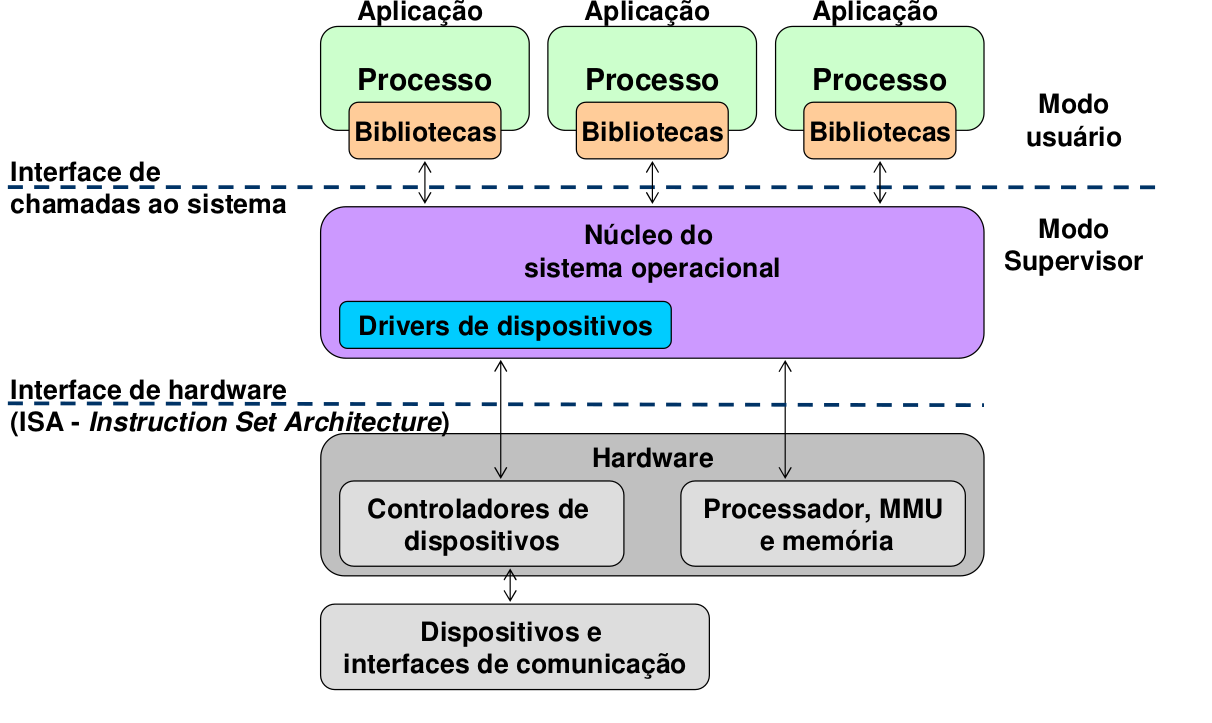
\includegraphics[width=0.7\textwidth]{assets/aula-tads-sope/aula-03-01.png}}
    
        \end{figure}
    \end{frame}
    \begin{frame}[fragile]{Sistemas Tradicionais: Multiprogramação}

        \begin{figure}[H]
            \centerline{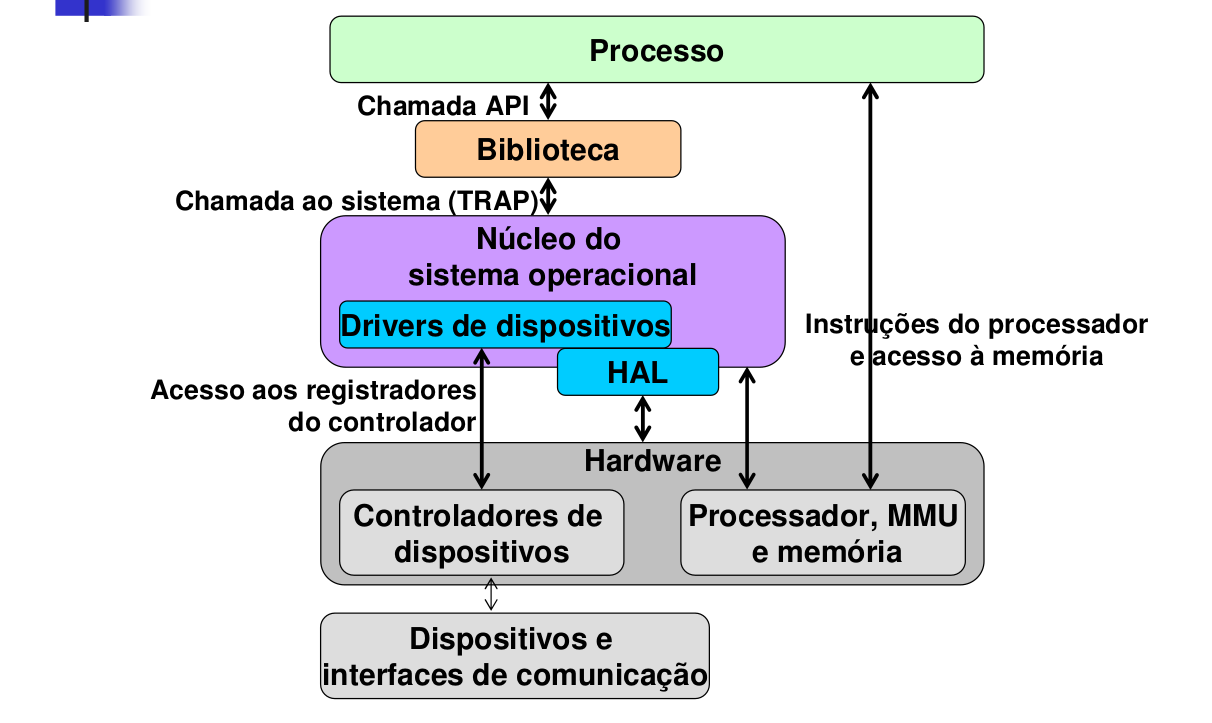
\includegraphics[width=0.7\textwidth]{assets/aula-tads-sope/aula-03-02.png}}
    
        \end{figure}
    \end{frame}
    
\section{Virtualização}
\begin{frame}{Virtualização}
    \begin{block}{Definição}
        Virtualização é um arcabouço ou metodologia de divisão de recursos de um computador em múltiplos ambientes de execução, através da aplicação de uma ou mais técnicas como particionamento de software e hardware, time-sharing, simulação parcial ou completa de máquina, emulação, qualidade de serviço e muitas outras.
    \end{block}
\end{frame}

\begin{frame}{Níveis de Virtualização}
    \begin{itemize}
        \item Nível da linguagem de programação
        \begin{itemize}
            \item Interpretação de uma linguagem ou instruções virtuais
        \end{itemize}
        \item Nível de biblioteca
        \begin{itemize}
            \item Chamadas ao sistema (system calls)
        \end{itemize}
        \item Nível de abstração de hardware
        \begin{itemize}
            \item User level API
        \end{itemize}
        \item Nível do sistema operacional
        \begin{itemize}
            \item HAL (Hardware Abstraction Layer)
        \end{itemize}
        \item Nível do conjunto de instruções
        \begin{itemize}
            \item ISA (Instruction Set Architecture)
        \end{itemize}
    \end{itemize}
\end{frame}

\begin{frame}{Virtualização ao Nível de HAL (Hardware Abstraction Layer)}
    \begin{itemize}
        \item Disponibiliza uma máquina virtual que corresponde a:
        \begin{itemize}
            \item Instruction Set Architecture (ISA)
            \item Virtualização dos dispositivos, processador e memória
        \end{itemize}
        
        \item Características:
        \begin{itemize}
            \item Host hóspede e hospedeiro utilizam a mesma ISA (Instruction Set Architecture)
        \end{itemize}

        \item Técnica utilizada:
        \begin{itemize}
            \item Mapeamento dos recursos virtuais sobre os recursos físicos
            \item Máquina virtual: Processamento (aplicações e sistema operacional) é realizado diretamente sobre o processador físico
            \item Instruções privilegiadas: são tratadas pelo sistema de virtualização
            \item Acesso a dispositivos: intermediado pelo sistema de virtualização
        \end{itemize}
    \end{itemize}
\end{frame}

\begin{frame}[fragile]{Virtualização de hardware}

    \begin{figure}[H]
        \centerline{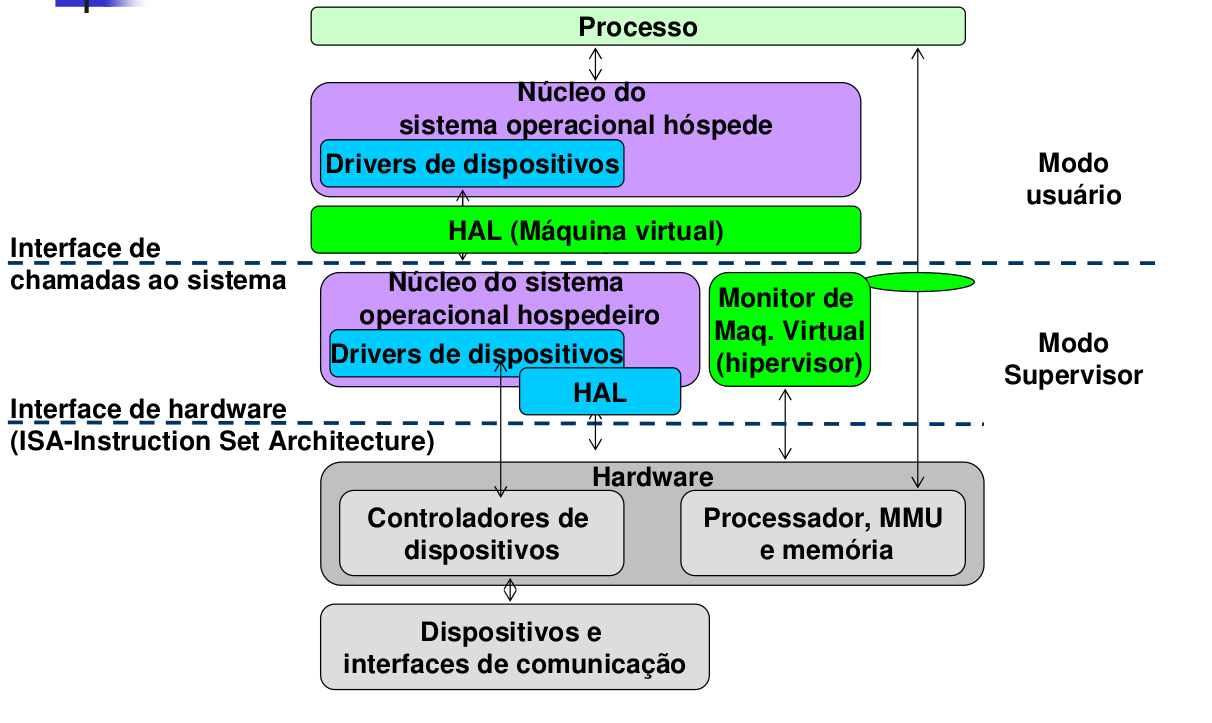
\includegraphics[width=0.7\textwidth]{assets/aula-tads-sope/aula-03-03.png}}

    \end{figure}
\end{frame}




\begin{frame}{Tipos de Sistemas de Virtualização}
    \begin{itemize}
        \item \textbf{Hosted}
        \begin{itemize}
            \item A virtualização é realizada com o auxílio de um sistema operacional hospedeiro.
        \end{itemize}

        \item \textbf{Stand alone (ou Bare Metal)}
        \begin{itemize}
            \item A virtualização é realizada sem auxílio de um sistema operacional hospedeiro.
        \end{itemize}
    \end{itemize}
\end{frame}

\begin{frame}[fragile]{Sistema tipo Hosted}

    \begin{figure}[H]
        \centerline{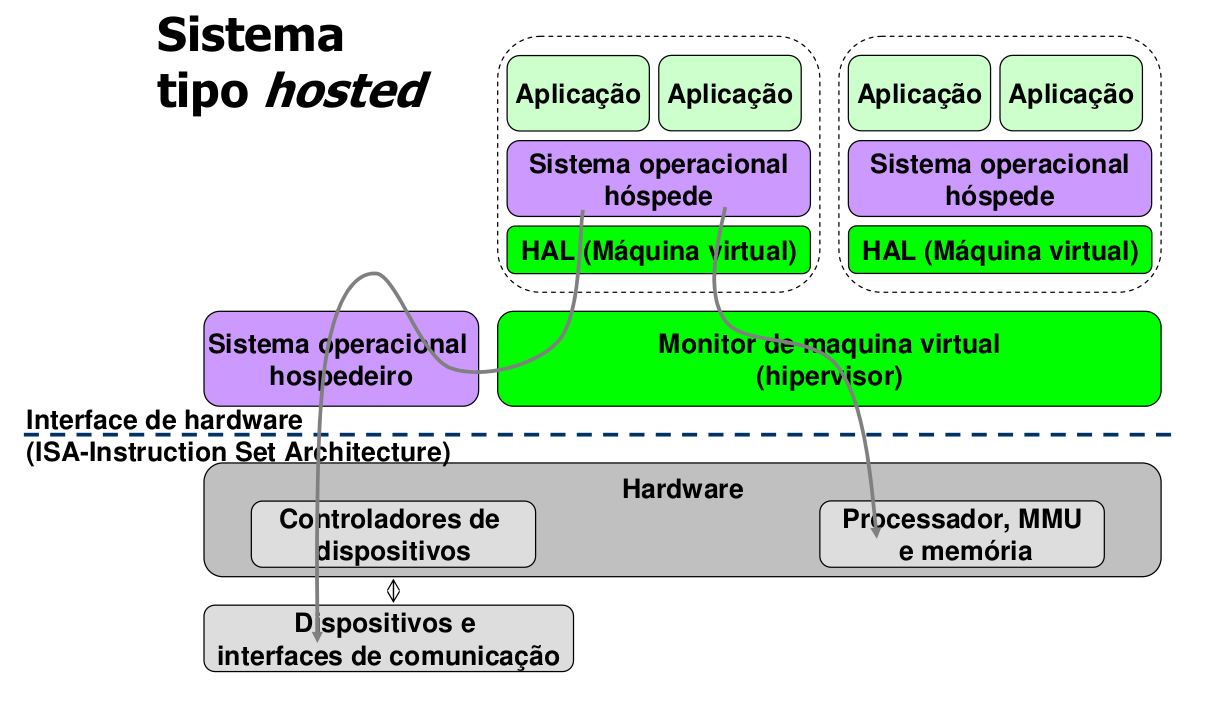
\includegraphics[width=0.7\textwidth]{assets/aula-tads-sope/aula-03-04.png}}

    \end{figure}
\end{frame}
\begin{frame}[fragile]{Baremetal}

    \begin{figure}[H]
        \centerline{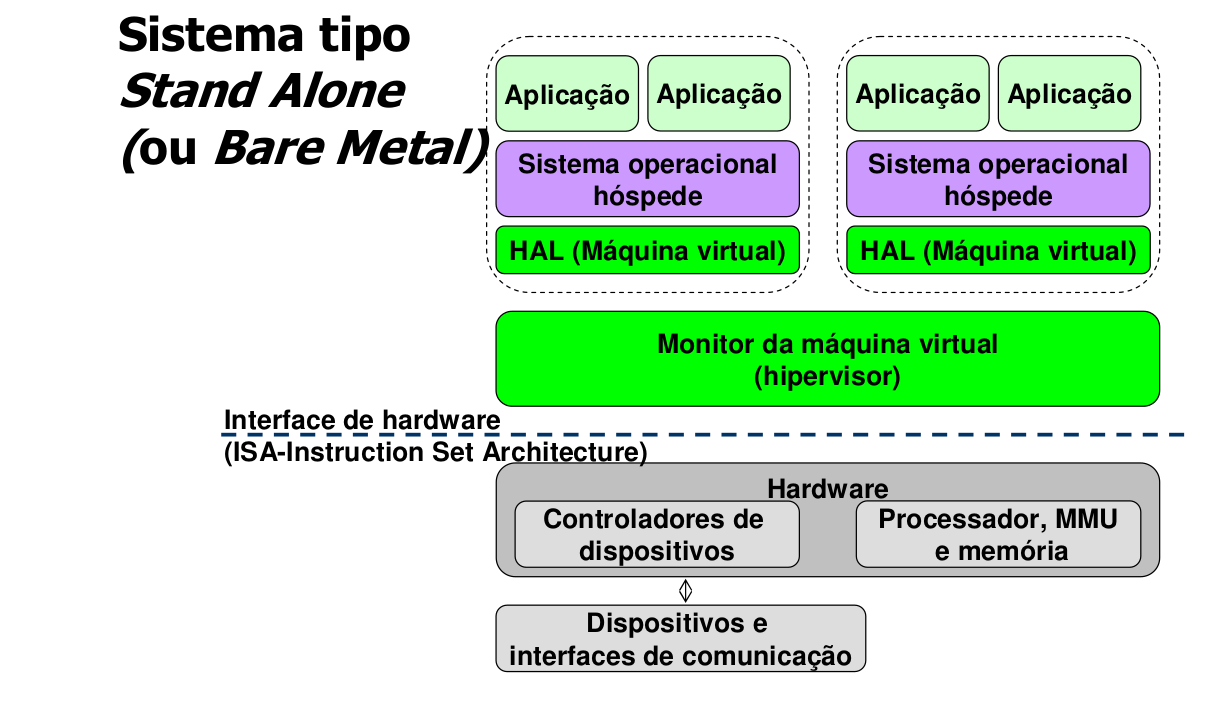
\includegraphics[width=0.7\textwidth]{assets/aula-tads-sope/aula-03-05.png}}

    \end{figure}
\end{frame}


\begin{frame}{Virtualização de Hardware}
    \begin{itemize}
        \item \textbf{Vantagens}
        \begin{itemize}
            \item Pouca sobrecarga (rápido)
            \item Isolamento e independência dos hosts hóspedes
            \item Possibilidade de utilização de diferentes sistemas operacionais nos hosts hóspedes
        \end{itemize}
        
        \item \textbf{Motivações para virtualização}
        \begin{itemize}
            \item Consolidação de servidores
            \item Ambientes de teste e homologação de sistemas
            \item Depuração de aplicações complexas e do sistema operacional
            \item Migração de sistemas
        \end{itemize}
        
        \item \textbf{Exemplos}
        \begin{itemize}
            \item VMware
            \item Xen
            \item VirtualBox
            \item Microsoft Hiper-V (Windows Server Virtualization)
        \end{itemize}
    \end{itemize}
\end{frame}

\begin{frame}{Sistemas de Virtualização de Servidores}
    \begin{itemize}
        \item Utilizam a técnica de virtualização HAL
        \item \textbf{Requisitos desejáveis}
        \begin{itemize}
            \item Sistema de armazenamento compartilhado (storage)
        \end{itemize}
        
        \item \textbf{Funcionalidades adicionais}
        \begin{itemize}
            \item Virtualização de componentes de rede
        \end{itemize}
        
        \item \textbf{Exemplos}
        \begin{itemize}
            \item VMware
            \item Xen
            \item VirtualBox
            \item Microsoft Hiper-V (Windows Server Virtualization)
        \end{itemize}
    \end{itemize}
\end{frame}
\begin{frame}{Sistemas de Virtualização de Servidores}
    \begin{itemize}
        \item \textbf{Principais motivações para virtualização}
        \begin{itemize}
            \item Consolidação de servidores
            \begin{itemize}
                \item Agrupar vários servidores virtuais em um conjunto reduzido de servidores físicos.
            \end{itemize}
            \item Consolidação de aplicações
            \item Ambientes de teste e homologação de sistemas
            \item Execução de aplicações que utilizam diferentes sistemas operacionais
            \item Migração de sistemas
            \item Provisionamento de servidores
            \item Recuperação de desastres
        \end{itemize}
    \end{itemize}
\end{frame}

\begin{frame}{Sistemas de Virtualização de Servidores}
    \begin{itemize}
        \item \textbf{Terminologia}
        \begin{itemize}
            \item Sistema operacional hóspede e hospedeiro
            \item Tipos de virtualização HAL
            \begin{itemize}
                \item Virtualização total
                \item Paravirtualização
            \end{itemize}
            \item Máquina Virtual (MV)
            \item Hypervisor ou monitor de máquina virtual (MMV)
        \end{itemize}
    \end{itemize}
\end{frame}
\begin{frame}{Sistemas de Virtualização de Servidores}
    \begin{itemize}
        \item \textbf{Sistema operacional hóspede}
        \begin{itemize}
            \item Sistema operacional que executa sobre uma máquina virtual
        \end{itemize}
        
        \item \textbf{Sistema operacional hospedeiro}
        \begin{itemize}
            \item Sistema operacional que executa diretamente sobre a máquina real
            \item Utilizado como infra-estrutura para criação das máquinas virtuais
        \end{itemize}
    \end{itemize}
\end{frame}
\begin{frame}{Sistemas de Virtualização de Servidores - Virtualização Total}
    \begin{itemize}
        \item \textbf{Virtualização total}
        \begin{itemize}
            \item A virtualização ocorre sem a inclusão de otimizações ao Sistema Operacional para virtualização.
            \item Gera certa quantidade de sobrecarga pois o Monitor de Máquina virtual deve oferecer à Máquina Virtual uma imagem semelhante a um sistema real, incluindo:
            \begin{itemize}
                \item BIOS virtual
                \item Espaço de memória virtual
                \item Gerenciamento de memória virtual
                \item Dispositivos virtuais
            \end{itemize}
        \end{itemize}
    \end{itemize}
\end{frame}
\begin{frame}{Sistemas de Virtualização de Servidores - Para-virtualização}
    \begin{itemize}
        \item \textbf{Para-virtualização}
        \begin{itemize}
            \item Técnica de virtualização onde o sistema operacional hóspede é modificado para otimizar o desempenho.
            \item A máquina virtual HAL é similar, porém não idêntica àquela do hardware real.
            \item Aumenta o desempenho da execução na máquina virtual.
        \end{itemize}
    \end{itemize}
\end{frame}
\begin{frame}{Sistemas de Virtualização de Servidores - Máquina Virtual e Hypervisor}
    \begin{itemize}
        \item \textbf{Máquina Virtual (ou Domínio)}
        \begin{itemize}
            \item Ambiente que é virtualizado, correspondendo ao sistema operacional e aplicações deste sistema operacional.
        \end{itemize}
        
        \item \textbf{Monitor de Máquina Virtual (Hypervisor)}
        \begin{itemize}
            \item Responsável pelas atividades de gerenciamento dos recursos da máquina virtual.
        \end{itemize}
    \end{itemize}
\end{frame}




\begin{frame}{Referências }\justifying
    \begin{itemize}
        \item \textbf{Slides SOPA2 - Prof. Alexandre Beletti Ferreira}
        \item \textbf{TANENBAUM, Andrew S.; WOODHULL, Albert S.} Sistemas operacionais: projeto e implementação. 3. ed. Porto Alegre: Bookman, 2008. ISBN 9788577800571.
    \end{itemize}
\end{frame}


\begin{frame}[fragile]{Imagem do dia}

    \begin{figure}[H]
        \centerline{
\includegraphics[width=0.3\textwidth]{assets/imagem-do-dia/docker-meme.jpeg}}

    \end{figure}
\end{frame}

\backmatter
\end{document}
